% Template for ICIP-2012 paper; to be used with:
%          spconf.sty  - ICASSP/ICIP LaTeX style file, and
%          IEEEbib.bst - IEEE bibliography style file.
% --------------------------------------------------------------------------
\documentclass{article}
\usepackage{spconf,amsmath,graphicx}

% Example definitions.
% --------------------
\def\x{{\mathbf x}}
\def\L{{\cal L}}

% Title.
% ------
\title{A Model for Solving Infinitely Repeated 2-Player Cournot Games}

\name{Fangzhu Yang, Tim Hu, Jaemo Lee}
\address{Brandeis University}
\begin{document}
%\ninept
%
\maketitle
%
\begin{abstract}76y
Infinitely iterated games have different Nash equilibrium sets than finite games. Cournot games are a common business model in a duopoly market. Our project aims to simulate infinitely repeated Cournot games and solve for the subgame-perfect Nash equilibrium sets. In order to achieve this, we use a simpler version of the Abreu-Pearce-Stachetti (APS) algorithm and build the operator R function that they wrote of within their paper. After applying the operator R on the original feasible payoff set for \textit{n} times, the set of payoffs eventually converges to what is essentially the Nash equilibrium set, $V^*$. 
\end{abstract}
%
\begin{keywords}
APS algorithm, Computational economics, Cournot games,  Economic modeling, Game theory, Game theory modeling, Infinitely repeated games, Iterated games,  Nash equilibrium
\end{keywords}
%
\section{Introduction}
\label{sec:intro}

Our research's purpose is to construct an algorithm for solving two-player infinitely repeated games and to compute the set $V^*$ of payoff pairs of all pure-strategy subgame-perfect Nash Equilibria. In this paper, we specifically focus on the Cournot game. For simplificiation purposes, we have two players who can choose to supply three discrete levels of quantity: low, medium or high level. 
	
	In a one-stage game, there exists a unique Nash equilibrium for that game. The same is true for a finitely repeated game. This can be proved through the use of of backwards induction. Unlike the rest, an infinitely repeated game does not arrive at a unique Nash equilibrium. As the game is played infinitely, we cannot apply backwards induction, resulting in no unique equilibrium point. 
	
	In game theory, possible Nash equilibrium payoff profiles in repeated games are discussed within \textit{The Folk Theorem} . It argues that the Nash equilibrium in a one-shot game is always for the players to choose the selfish strategy that is in their most interest, however, in the infinitely repeated game players tend to cooperate, given that they are sufficiently patient. Infinitely iterated games are incredibly relevant. In reality, it is often unknown to us when exactly a game is going to end. Therefore, most real life situations can be modeled as an infinitely repeated game. The discount factor plays an important role in infinitely repeated games, indicating a player's patience. The higher a discount rate is, the more patient the player is, and the more likely that a cooperative action will be picked by a player.
	
	Our paper will focus on a simple repeated Cournot game, and solve for the subgame-perfect Nash Equilibria. Throughout our paper we will reference models based off the below payoff chart. The data represents an industry structure in which companies compete on the amount of output they will produce, which they decide on independently of each other and at the same time. We will show in our paper that cooperation can be achieved in the infinitely repeated Cournot game, with both players choosing medium production. 
	

\begin{figure}[!ht]

\begin{minipage}[b]{1.0\linewidth}
  \centering
  \centerline{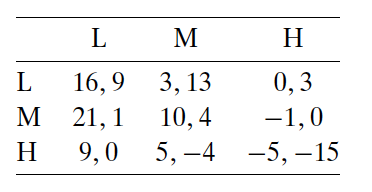
\includegraphics[width=4.75cm]{payoff}}
\end{minipage}
\caption{The payoff matrix for the simple Cournot game}
\label{fig:res}
%
\end{figure}

\section{The Algorithm}
\label{sec:format}

In Abreau and Sannikov's survey paper, the authors construct an algorithm that is related to the APS algorithm, while also more efficient and simpler to program.\cite{direct}\cite{survey}\cite{comp} We are going to use this Abreu and Sannikov algorithm for our project to solve for the iterated Cournot game. The key to this algorithm is the R operator. Due to their close nature, it is helpful to first have an understanding of the APS algorithm. 

\subsection{the APS Algorithm}
\label{ssec:subhead}
	
	Let g(a) denote the payoff the the action profile and P(X) denote the worst punishment for each player. h(a) denotes the maximum payoff that the player can get by deviating from the one-stage equilibrium. The APS algorithm uses these variables to construct the operator B as follows: 
	
	B(W) = co$\{$v $\mid$ $\exists$ w $\in$ W, a $\in$ A s.t. v = (1 - $\delta$)g(a) + $\delta$w and $\delta$(w - P(W)) $\geq$ (1 - $\delta$)h(a)$\}$
	
	This definition can be decomposed into two parts:
	
	The first part \textit{v = (1 - $\delta$)g(a) + $\delta$w} is adding the current payoff and continuation value. 
	
	The second part \textit{$\delta$(w - P(W)) $\geq$ (1 - $\delta$)h(a)} is the incentive constraint,  (IC). It is used to guarantee that each player prefers her equilibrium action over deviating and receiving her worst equilibrium punishment. 

	When the two conditions are satisfied, we can construct the operator B. So, if we define $W^n$ = B(W$^{n-1}$) recursively, than the APS algorithm shows that:
	
\begin{center}
$W^n$ $\rightarrow$ $V^*$ as n $\rightarrow$ $\infty$
\end{center}

	Starting from the original feasible set $W^0$, we can get the Nash equilibrium set $V^*$ after a large number of iterations. However, after adopting this algorithm for our project, we were faced with one big problem. Because of the number of vertices that the sets of the sequence ${W^n}$ produce, the number of vertices could potentially grow without bound, the APS algorithm does not yield a bound on the number of extreme points of $V^*$. 
	
\subsection{Constructing operator R}
\label{ssec:subhead}
	
	To make the computation simpler, we instead construct the operator R, where at most 4 $\mid$A$\mid$ extreme points of $V^*$ are generated ($\mid$A$\mid$ is the number of stage game action profiles). Thus, the R operator simplifies our computation by a large scale.  The definition for operator R is as follows:
	
	For an action profile \textit{a}, a convex set W, and a punishment vector u (u is always equal to 0 in our algorithm), we can define C(a,W, u) = ${g(a)}$ if $\delta$(g(a) - u) $\geq$ (1 - $\delta$)h(a), otherwise, let $\delta$($w_1$ - $u_1$) = (1 - $\delta$)$h_1(a)$ or $\delta$($w_2$ - $u_2$) = (1 - $\delta$)$h_2(a)$. Therefore,
	
	
\begin{center}
	R(W, u) = co$\cup$(1 - $\delta$)g(a) + $\delta$C(a, W, u)
\end{center}
	
	Notice that for any a $\in$ A, the operator R considers at most four extreme points. Based on the successive applications of this operator, our algorithm can lead us to the final Nash equilibrium set $V^*$. 
	

\begin{figure}[htb]

\begin{minipage}[b]{1.0\linewidth}
  \centering
  \centerline{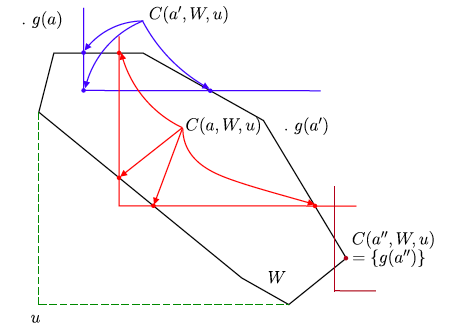
\includegraphics[width=5.5cm]{roperator}}
\caption{C(a, W, u)}
\label{fig:res}
\end{minipage}
\end{figure}

\section{Implementation}
\label{implement}
We created a graphic user interface function to help out people who are not familiar with scripting easier access to the information provided by our model. The GUI is constructed with the GUIDE process within Matlab to set the positions and sizes of each toolbox in order. We used an axes to plot the figure of each iteration set, 9 radio buttons which are associated with each action profile and one more extra button to show all of the lines and extreme points with the boundary and vertex intersection points, a UI toolbox to control the buttons, a slider to prompt each iteration of the plot, and the edit text box to display the iteration status and manually handle the slider bar. 

When the program is ran, the initial image of the GUI is shown below:

\begin{figure}[htb]
\begin{minipage}[b]{1\linewidth}
  \centering
  \centerline{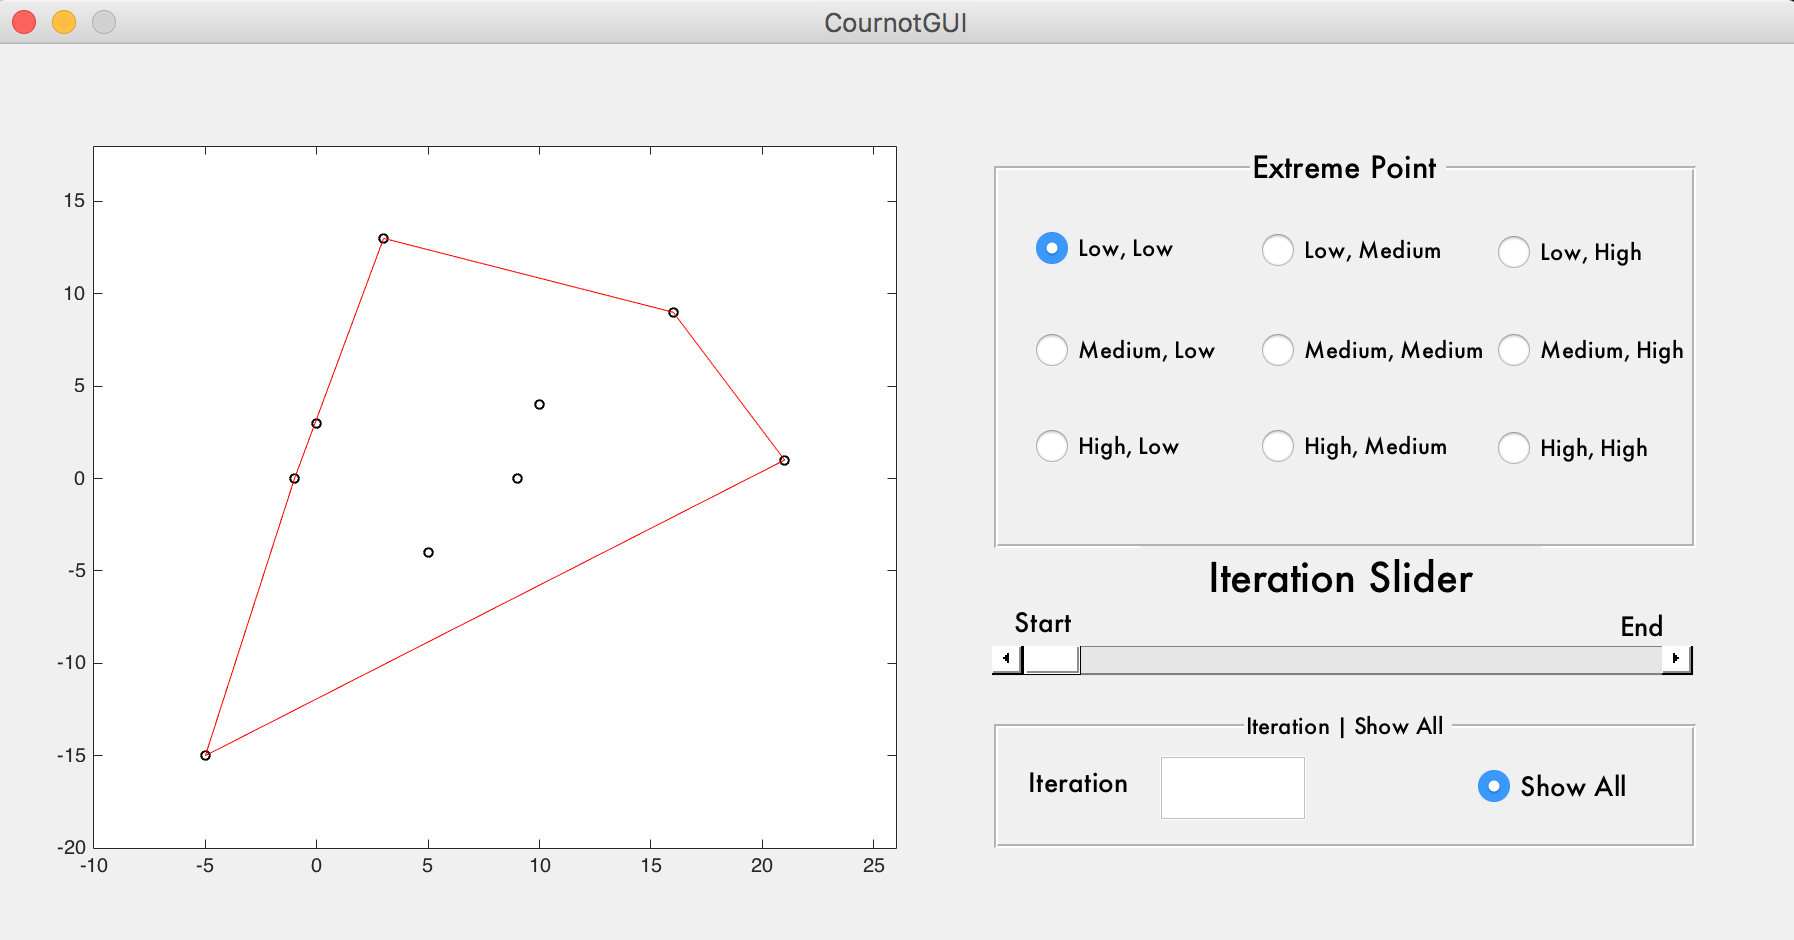
\includegraphics[width=6cm]{GUI1}}
  \centerline{(a) The starting GUI}\medskip
\end{minipage}
\hfill
\begin{minipage}[b]{1\linewidth}
  \centering
  \centerline{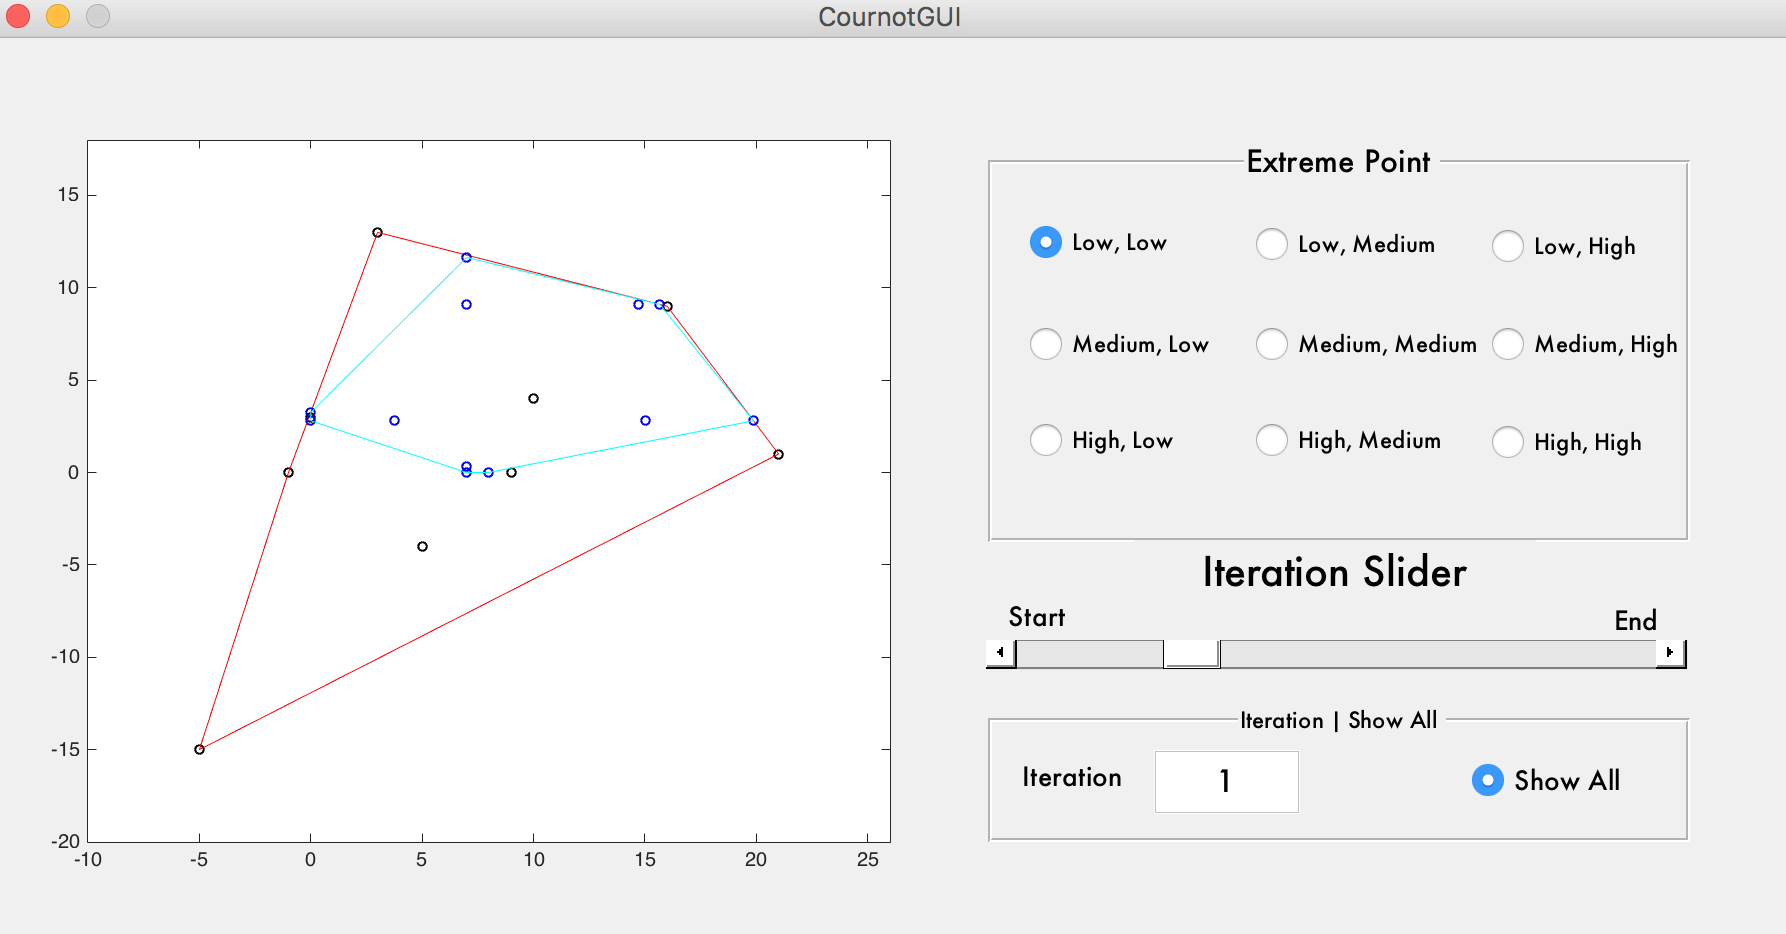
\includegraphics[width=6cm]{GUI2}}
  \centerline{(b)  An example of an iteration's potential payoffs}\medskip
\end{minipage}
\hfill
\end{figure}
The program traverses each iteration with the slider bar. The text box on the left bottom shows the amount of iterations for said model. The user can type the number in it and move the slider for different iteration plots. Each radio button is associated with the payoff option and when it is clicked on, it shows the lines connecting the respective extreme points and the intersection points including ones with the boundary and the vertex. Since the plot is reassigned each time the radio button is clicked, to use the different option, the slider bar has to be be clicked again.

\begin{figure}[htb]

\begin{minipage}[b]{1\linewidth}
  \centering
  \centerline{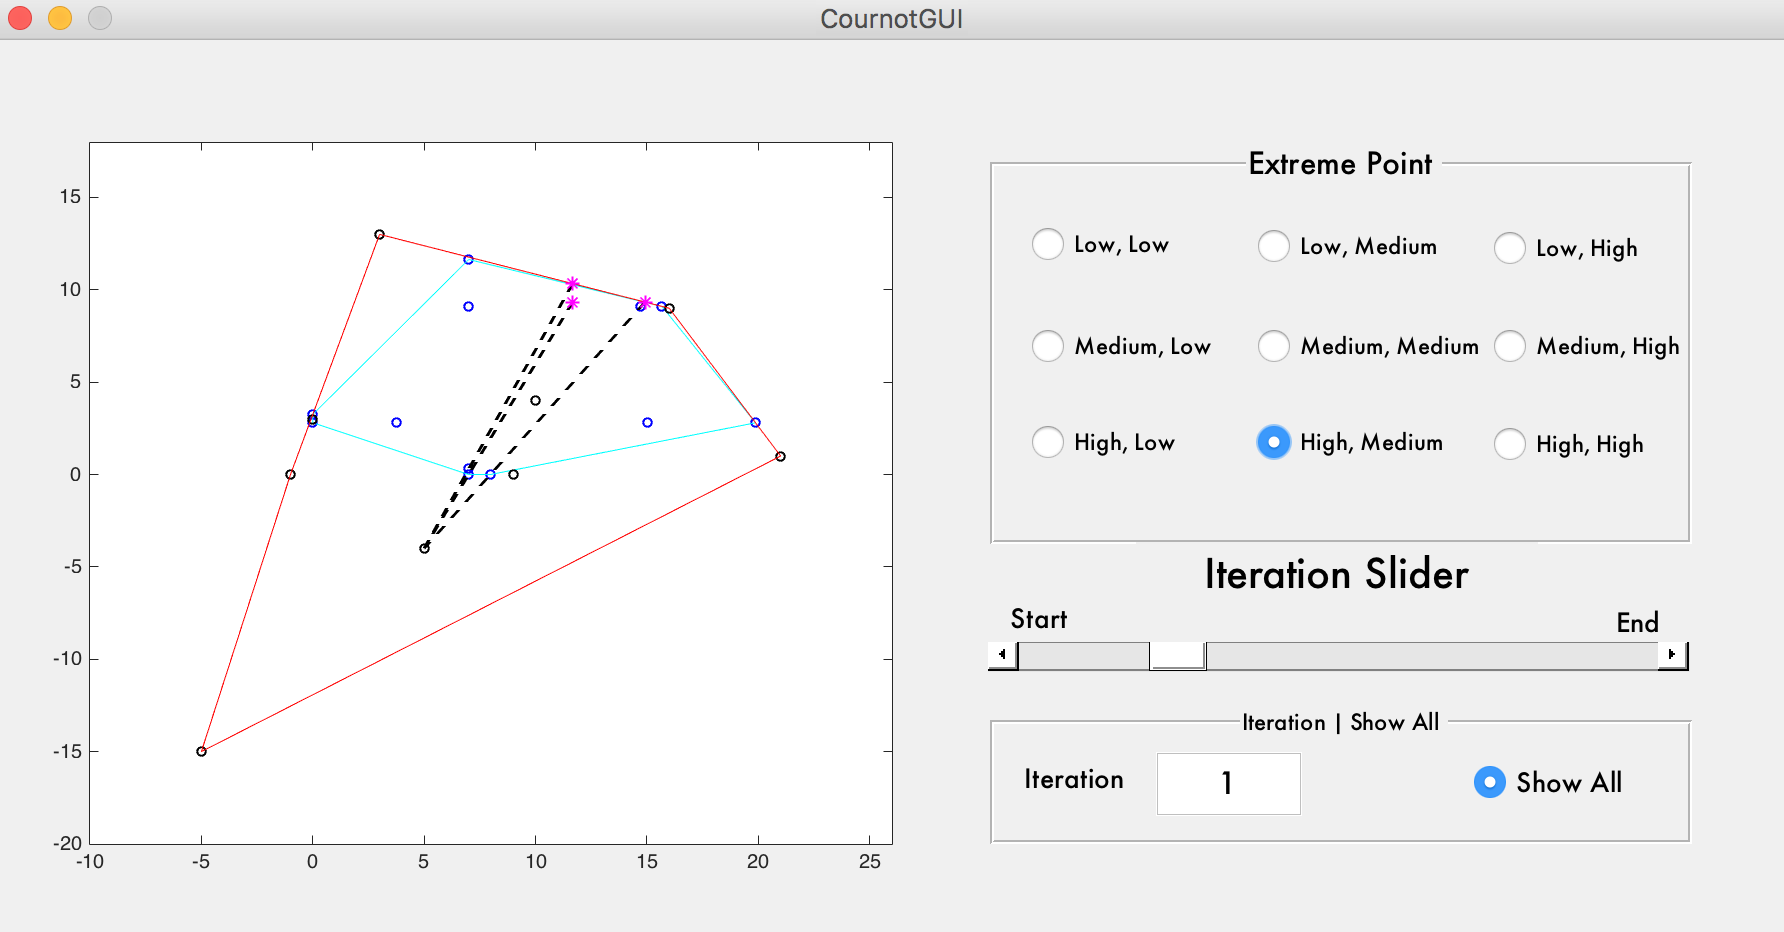
\includegraphics[width=6cm]{GUI3}}
  \centerline{(c) The starting GUI}\medskip
\end{minipage}
\hfill
\begin{minipage}[b]{1\linewidth}
  \centering
  \centerline{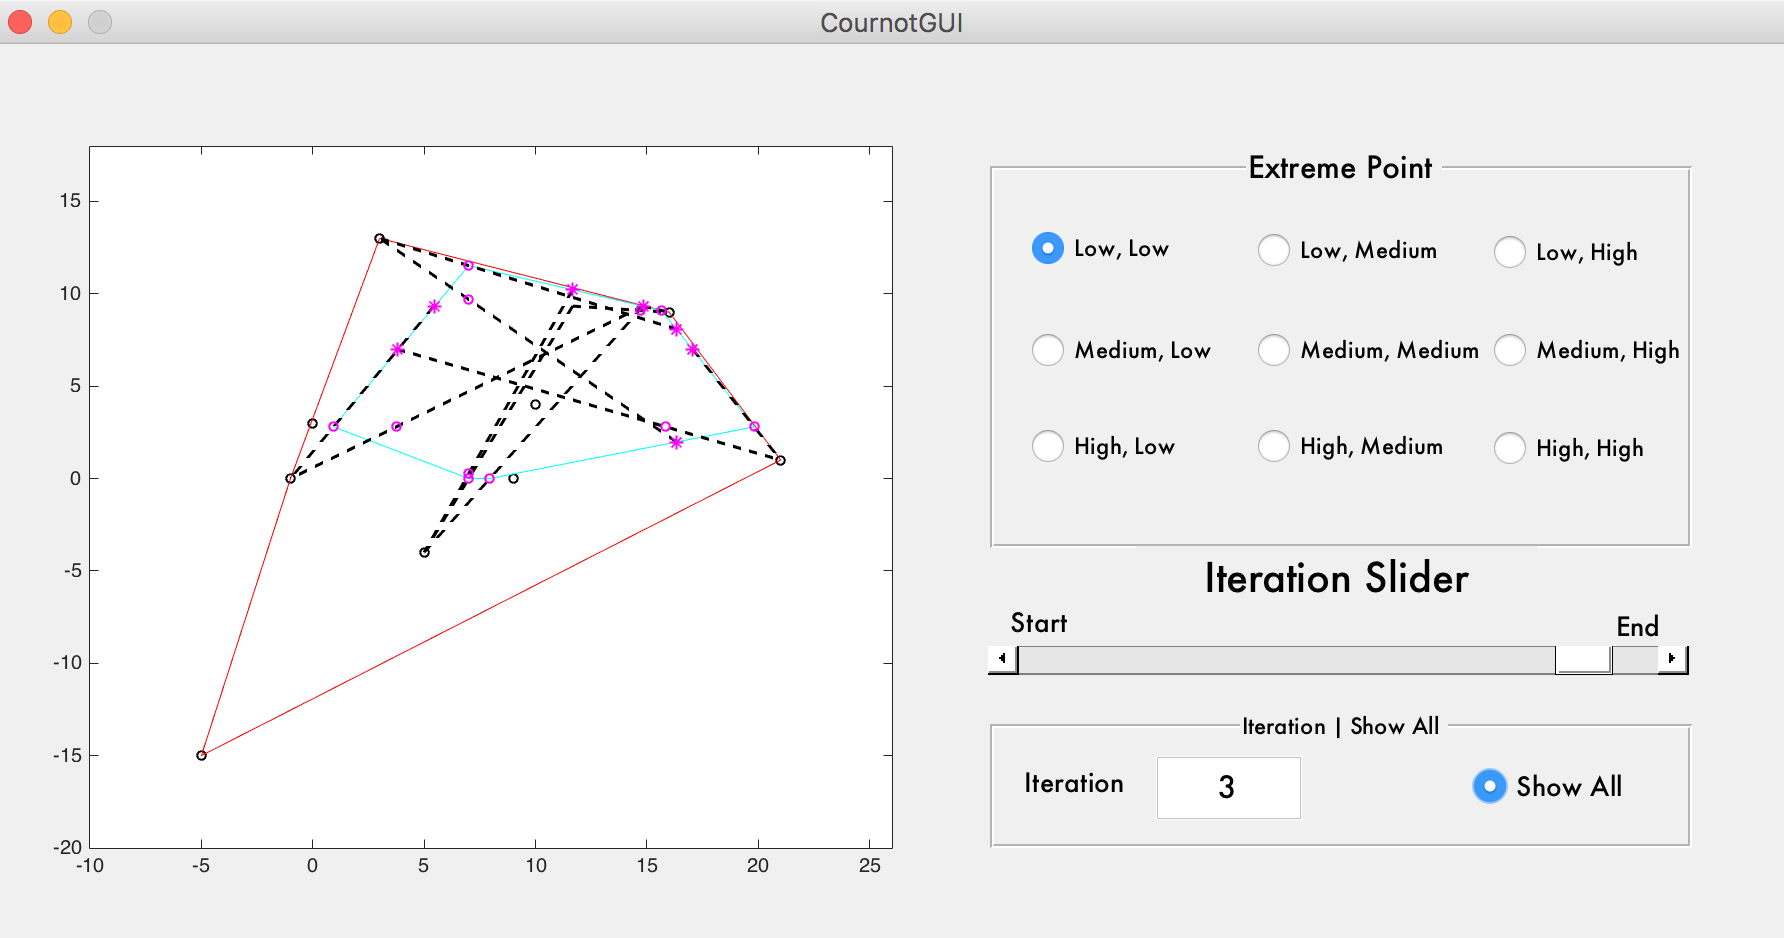
\includegraphics[width=6cm]{GUI4}}
  \centerline{(d) An example of an iteration's potential payoffs}\medskip
\end{minipage}
\caption{Example of the GUI implementation.}
\label{fig:res}

\end{figure}
Three parts constitute the programming within the GUI: opening function, slider callback, and radio buttons. We first input the main algorithm into the opening function so that when the GUI is opened the user can see the feasible set. All the data used in the other functions are stored in the cell array named /textit{data} and each cell contains another cell with each iteration's data. It is similar to a map data structure. The data cell array and other variables are shared by the global- prefix. The data retrieved from the slider is stored in the sliderValue variable with the use of handle object. We set the minimum and maximum value of the slider and each slider step for setting the range of the slider moves when the user clicks on the arrow. When the user clicks on the middle part in-between the bar and the arrow, the plot will automatically change when the slider is changed each time the plot changes, the figure is cleared once to reset. sliderValue is also shared by the global prefix to be used in the text box to show the status and it is also used in the radio buttons as the iteration zero and the rest of the iterations have different numbers of the lines and extreme points. 

\section{Results and Applications}

We use the same data from Abreu and Sannikov's paper in order to be able to successfully compare Nash equilibriums derived using our model. The results produced from our model consist of a graph containing two polygons. The outer polygon is the set of all possible action profiles from the original payoff chart. One can see that the black circles in figure 5 mirror the payoffs. Player 1 is on the x-axis, and player 2 is on the y-axis. The inner polygon consists of all possible payoffs that would potentially satisfy an iterated game. Because only one action profile exists within the inner polygon, that is the optimal payoff structure for our game. Knowing this allows for greater efficiency in making a decision. If both players knew this prior to entering a 'game', fewer costs would be met through better mutually beneficial decisions. Below are our inputs and outputs.

\begin{figure}[!ht]
\begin{minipage}[b]{1.0\linewidth}
  \centering
  \centerline{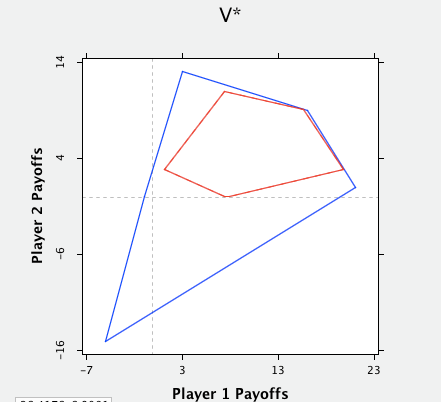
\includegraphics[width=5.5cm]{V-Star}}
\caption{Set of Nash Equilibrium Points}
\label{fig:res}
\end{minipage}
%
\end{figure}

\begin{figure}[!ht]

\begin{minipage}[b]{1.0\linewidth}
  \centering
  \centerline{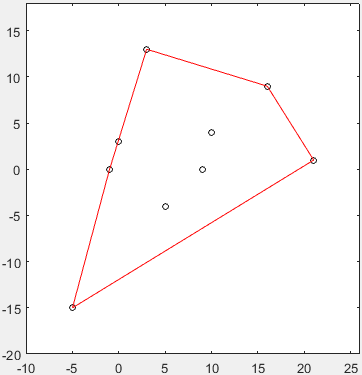
\includegraphics[width=5.5cm]{FeasibleSet}}
\caption{ The polygon formed with the feasible set.}
\label{fig:res}
\end{minipage}
%
\end{figure}
In addition, our model generates a lot of useful data. Each operator point is related to an initial payoff and can describe potential payoffs outcomes in the future with different patience levels. All rewards along the line of each relation can be accessed with different patience levels. This is helpful in helping players understand how they discount the future impact their long-run reward.

\begin{figure}[!ht]
\begin{minipage}[b]{.48\linewidth}
  \centering
  \centerline{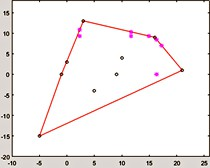
\includegraphics[width=3.75cm]{OperatorPoints}}
\centerline{(a) Operator Points}\medskip
\end{minipage}
\hfill
\begin{minipage}[b]{0.48\linewidth}
  \centering
  \centerline{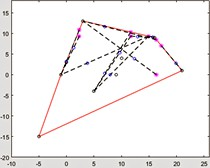
\includegraphics[width=3.75cm]{applyingDiscountFactor}}
\centerline{(b) Payoff-Operator w/ discount factor}\medskip
\end{minipage}
%
\caption{Algorithm steps }
\label{fig:res}
%
\end{figure}

Next, we can also see each iteration's possible payoffs. This is useful if a player does not plan to play until the nash equilibrium and is more interested in the short-term.

\begin{figure}[!ht]
%
\begin{minipage}[b]{.48\linewidth}
  \centering
  \centerline{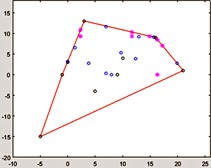
\includegraphics[width=3.75cm]{newPoints}}
  \centerline{(c) Next iteration's payoffs}\medskip
\end{minipage}
\hfill
\begin{minipage}[b]{0.48\linewidth}
  \centering
  \centerline{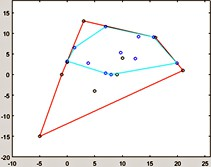
\includegraphics[width=3.75cm]{newPolygon}}
  \centerline{(d) Iteration 1 payoff structure}\medskip
\end{minipage}
%
\caption{Algorithm steps }
\label{fig:res}
%
\end{figure}

\section{Issues and future study}

Our project touches on the subject of computational methods to model iterated games. In addition, our project encountered issues within creating a more universal model for solving all forms of games. Initially, when we read the Abreu Sannikov paper, we wished to form a Matlab implementation similar to theirs that could solve for all types of games. In order to save time, we decided to focus on building a model for Cournot games only. That means certain payoff charts do not work with our model framework. In real life, there are situations where cooperation grows, meaning more viable payoffs. Our model determines the nash equilibrium by looking at the shrinkage of possible payoffs, incorrectly mentioned said situations.

Future studies can involve building more complex or more encompassing models. Our model stops at a simple 2 player iterated game. This model could be complicating by allowing for multiple dimensions, representing multiple players. The model could also be modified to specific industries based on empirical market data. Players often have different patience levels and that could be better modeled.

\section{Conclusion}

Our project started with the goal to form models for iterated games through Matlab. At the end, we were successful in computing models for an iterated 2-player Cournot game. We were able to successfully reproduce the results from the Abreu Sannikov paper. We implemented our own version of their ABS algorithm. Finally, we also produced our own GUI for better accessing the data within our code. If work were to continue on this project, we hope to see improvements made to our model that allow for different games and more complex relations.

\bibliographystyle{IEEEbib}
\bibliography{reference}

\end{document}

















